\chapter{CSV Document}
\label{csvDocument}

\begin{figure}[h!]
	\centering
		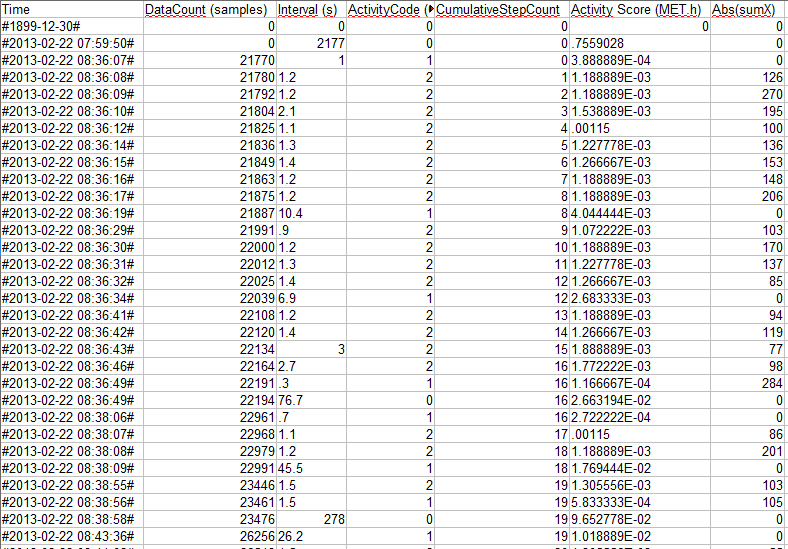
\includegraphics[width=1\textwidth]{csv.png}
		\caption[CSV Document]{\footnotesize The CSV document as seen in Libre Calculator}
		\label{fig:csvExtract}
\end{figure}

\begin{table}[h!]
  \centering
  \begin{tabular}{|l|p{8.4cm}|}
    \hline
    \textbf{Row Title} & \textbf{Description} \\ \hline
    Time & Time when the state started. \\ \hline
    DataCount & The amount of sensor readings the event interval is based on (not used in this project). \\ \hline
    Interval & Duration for the event interval presented in seconds. \\ \hline
    ActivityCode & Represents the activity of the user either sedentary (0), standing (1), or walking (2). \\ \hline
    CumulativeStepCount & The total amount of steps taken since movement tracking was started (not used in this project). \\ \hline
    Activity Score & Activity score rating (not used in this project) \\ \hline
    Abs(sumX) & Acceleration intensity (not used in this project). \\ \hline
  \end{tabular}
  \caption{A short description of the rows in figure~\ref{fig:csvExtract}.}
  \label{tab:csvDescription}
\end{table}
